\section{Activity Diagram}

\begin{figure}[!h]
    \centering
    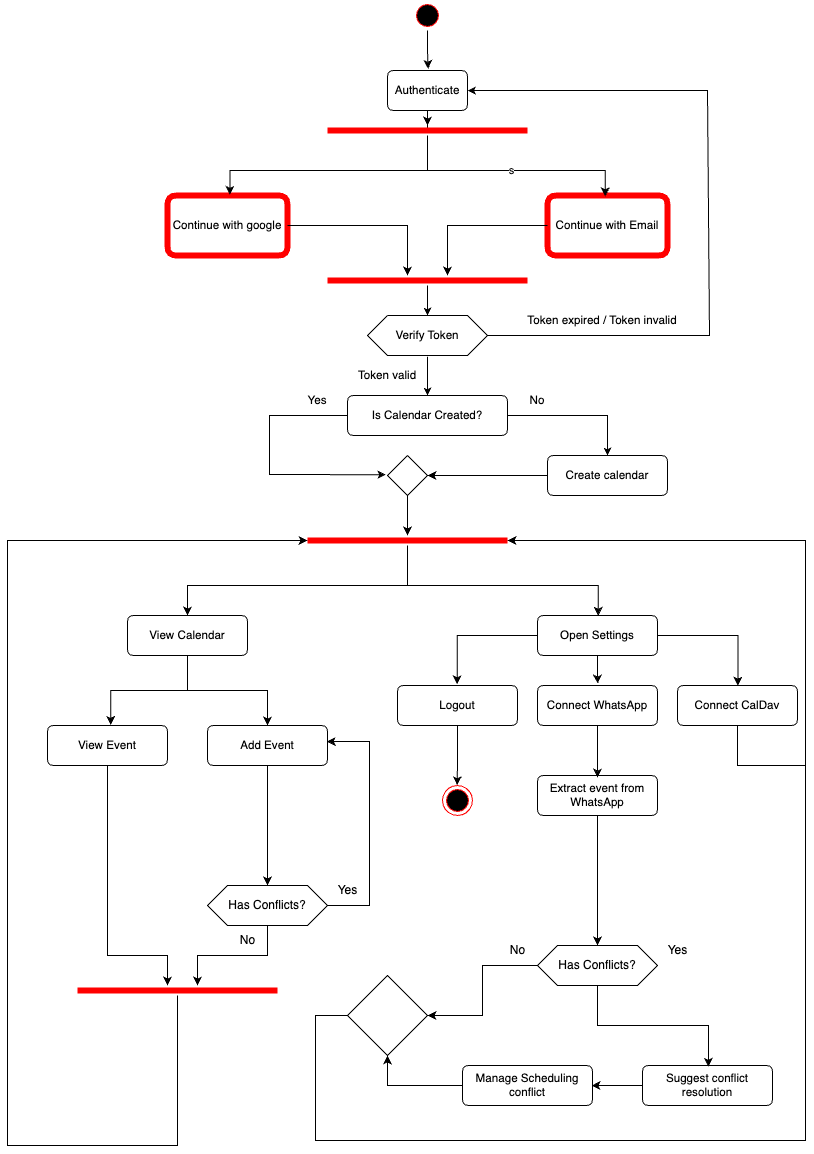
\includegraphics[width=0.9\textwidth]{images/activity-diagram.png}
    \caption{Activity Diagram of Jadwal}
    \label{fig:activity-diagram}
\end{figure}

\newpage

An activity diagram is shown in Figure~\ref{fig:activity-diagram} above, and it illustartes the flows the user of the app can take. It starts with the authentication whcih supports both Google and Email. Then afater the token is verified, a check is done to see if the user has a calendar or not. If the user has a calendar, we just move on, but if they don't have one, we create one and then move on. Here the user is inside the app and has two options, he can either view the calendar or open the settings page. When he views the calendar, he can view an event, or add one. Adding event might result in a conflict, so if one arises, they can try editing it and adding it again til no conflicts arise. After any of those two steps, the user can go back to view calendar or open settings page. If the choose to open settings page, they have three actions available. They can connect a CalDAV account, connect WhatsApp, or logout. Starting with the connecting a WhatsApp account, the system will extract events from the user's WhatsApp account automatically. If any conflicts arise, the system suggests a conflict resolution, and the user can take action by managing the scheduling conflict. But if no conflicts arise, the system just continues normally. Another option for the user is connecting a CalDAV account, and once that happens, the user can go back to having the option of going to calendar view or open settings page. Finally, the logout action and that terminates the session and the user is logged out of the app.

